\section{Results}

Our results provide three nested layers of evidence for the hallucination-type mechanism.

\subsection{Distributional Evidence: Token Probability Peakedness (h-m1)}

On LLaMA-2-7B TriviaQA, hallucinated responses show mean peakedness ratio of \textbf{2.936} vs.\ \textbf{2.533} for correct responses (two-sample $t$-test, $p = 0.002$, $n = 488$). Figure~\ref{fig:peakedness_kde} shows the KDE of peakedness distributions.

\begin{figure}[h]
\centering
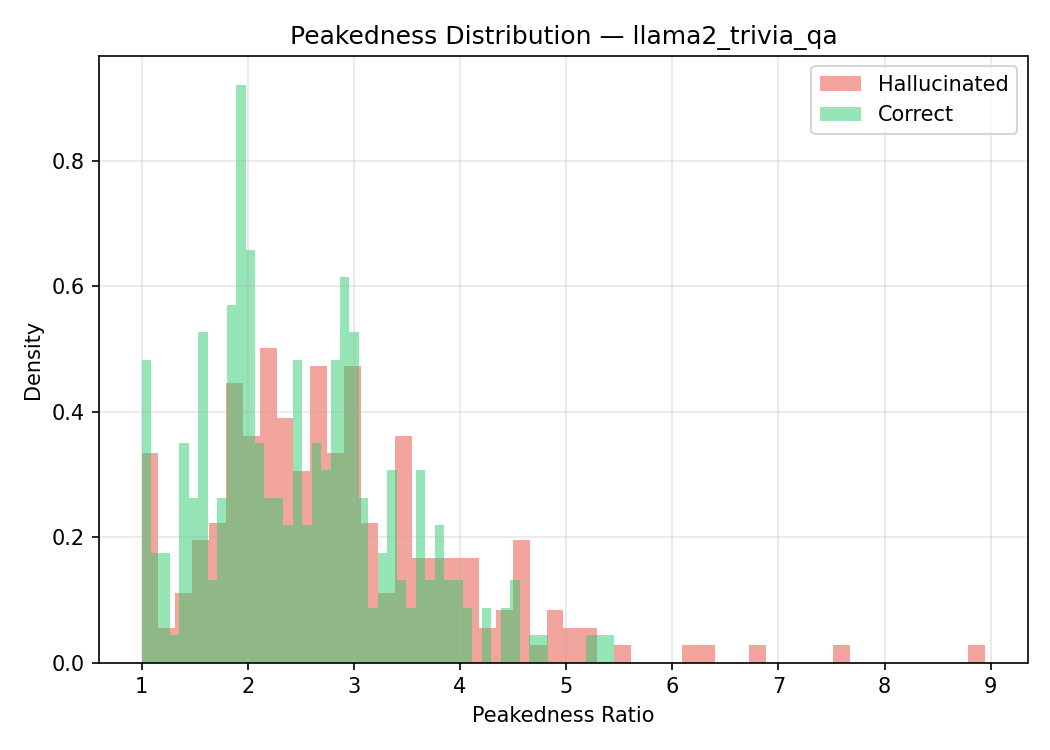
\includegraphics[width=0.9\columnwidth]{figures/peakedness_kde_llama2_trivia_qa}
\caption{KDE of token probability peakedness for hallucinated vs.\ correct responses on LLaMA-2-7B TriviaQA. Hallucinated responses show significantly higher peakedness ($p=0.002$).}
\label{fig:peakedness_kde}
\end{figure}

This establishes Step 1 empirically: recall-failure hallucinations produce significantly more peaked token probability distributions, converting the mechanism's distributional assumption into measured fact.

\subsection{Rank-Correlation Evidence: Aggregation Function Sensitivity (h-m2)}

\begin{table}[h]
\centering
\caption{Spearman $\rho$ for min and mean log-probability across model $\times$ dataset pairs. All four pairs confirm the predicted direction; all CIs exclude zero.}
\label{tab:rho}
\begin{tabular}{lllll}
\toprule
(Model, Dataset) & $\rho(\min)$ & $\rho(\text{mean})$ & $\Delta\rho$ & 95\% CI \\
\midrule
LLaMA-2-7B, TriviaQA & 0.604 & 0.397 & \textbf{+0.206} & [+0.147, +0.262] \\
Mistral-7B-v0.1, TriviaQA & 0.641 & 0.549 & \textbf{+0.092} & [+0.041, +0.143] \\
LLaMA-2-7B, TruthfulQA & 0.174 & 0.380 & \textbf{$-$0.206} & [$-$0.262, $-$0.147] \\
Mistral-7B-v0.1, TruthfulQA & 0.062 & 0.242 & \textbf{$-$0.180} & [$-$0.237, $-$0.123] \\
\bottomrule
\end{tabular}
\end{table}

All four (model $\times$ dataset) pairs show the correct direction; all four CIs exclude zero. The direction flip between TriviaQA ($\min > \text{mean}$) and TruthfulQA ($\text{mean} > \min$) is consistent across architecturally distinct models, confirming Step 2 at the signal level without threshold assumptions.

\subsection{AUROC Evidence: Threshold-Level Confirmation (h-m3)}

\begin{table}[h]
\centering
\caption{AUROC across models, datasets, and aggregation functions.}
\label{tab:auroc}
\begin{tabular}{lllll}
\toprule
Model & Dataset & AUROC(min) & AUROC(mean) & AUROC(raw\_sum) \\
\midrule
LLaMA-2-7B & TriviaQA & 0.849 & 0.730 & \textbf{0.896} \\
LLaMA-2-7B & TruthfulQA & 0.601 & \textbf{0.721} & 0.459 \\
Mistral-7B-v0.1 & TriviaQA & 0.892 & 0.836 & \textbf{0.895} \\
Mistral-7B-v0.1 & TruthfulQA & 0.538 & \textbf{0.649} & 0.417 \\
\bottomrule
\end{tabular}
\end{table}

\begin{figure}[h]
\centering
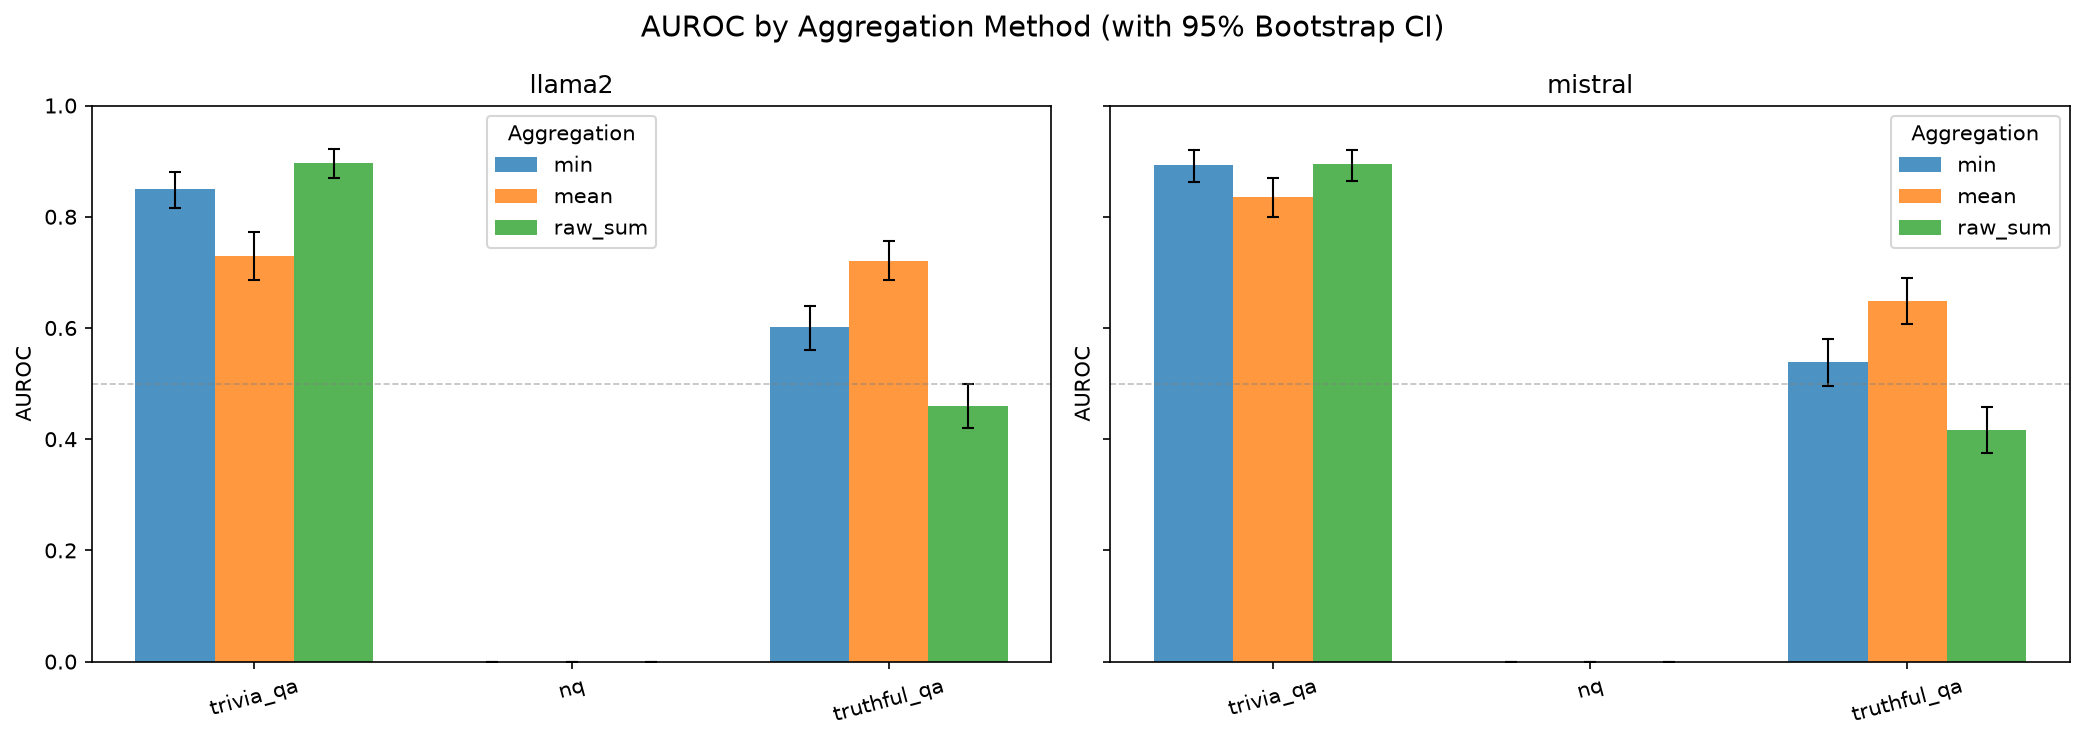
\includegraphics[width=\columnwidth]{figures/fig1_auroc_bar}
\caption{AUROC grouped bar chart with 95\% CI error bars across all model $\times$ dataset $\times$ aggregation combinations.}
\label{fig:auroc_bar}
\end{figure}

\begin{figure}[h]
\centering
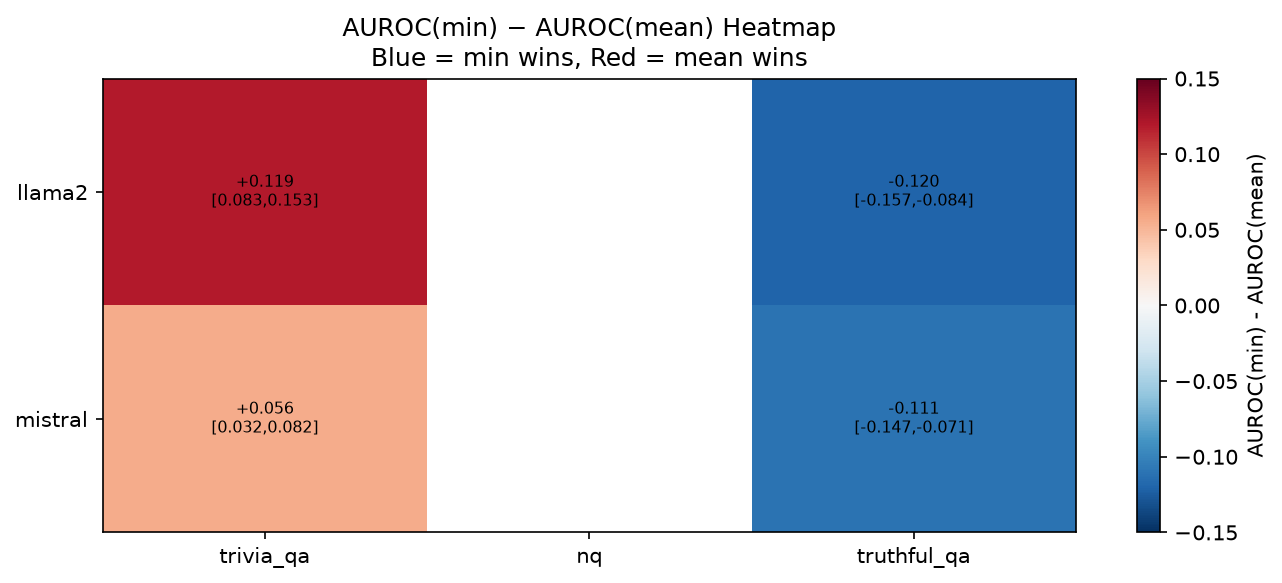
\includegraphics[width=0.85\columnwidth]{figures/fig2_diff_heatmap}
\caption{AUROC(min) $-$ AUROC(mean) heatmap. Positive values (blue) indicate min outperforms mean; negative (red) indicates mean outperforms min.}
\label{fig:diff_heatmap}
\end{figure}

\textbf{P1 (min $>$ mean on TriviaQA):}

\begin{table}[h]
\centering
\caption{P1 confirmation: $\Delta$AUROC(min$-$mean) on TriviaQA.}
\label{tab:p1}
\begin{tabular}{lll}
\toprule
Model & $\Delta$AUROC(min$-$mean) & 95\% CI \\
\midrule
LLaMA-2-7B & \textbf{+0.119} & [+0.083, +0.153] \\
Mistral-7B-v0.1 & \textbf{+0.056} & [+0.032, +0.082] \\
\bottomrule
\end{tabular}
\end{table}

P1 confirmed for both models. Effect size: 5--12 AUROC points.

\textbf{P2 (mean $>$ min on TruthfulQA):}

\begin{table}[h]
\centering
\caption{P2 confirmation: $\Delta$AUROC(mean$-$min) on TruthfulQA.}
\label{tab:p2}
\begin{tabular}{lll}
\toprule
Model & $\Delta$AUROC(mean$-$min) & 95\% CI \\
\midrule
LLaMA-2-7B & \textbf{+0.120} & [+0.084, +0.157] \\
Mistral-7B-v0.1 & \textbf{+0.111} & [+0.071, +0.147] \\
\bottomrule
\end{tabular}
\end{table}

P2 confirmed for both models with effect sizes of 11--12 AUROC points.

\begin{figure}[h]
\centering
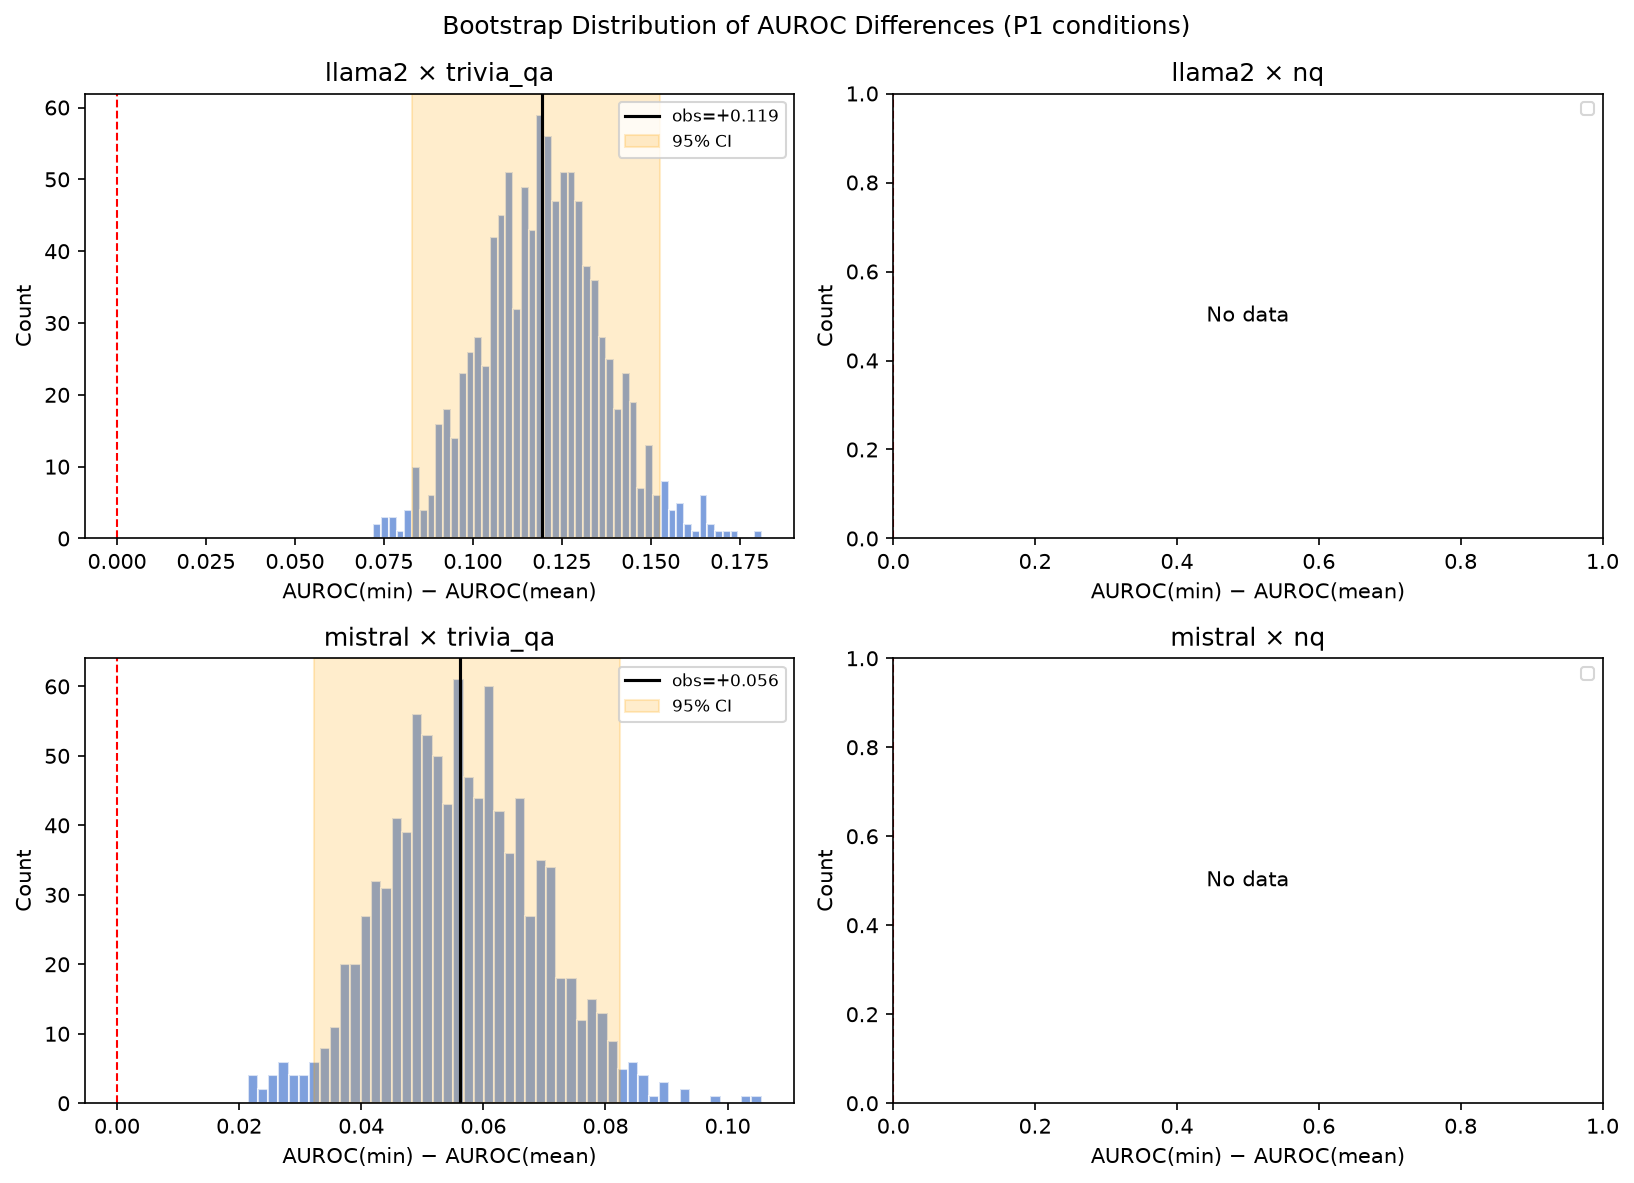
\includegraphics[width=\columnwidth]{figures/fig3_bootstrap_dists}
\caption{Bootstrap differential distributions for P1 and P2, confirming both are well-separated from zero.}
\label{fig:bootstrap_dists}
\end{figure}

\subsection{Unexpected Finding: Raw\_sum as Strongest Factual-Recall Detector}

Raw unnormalized log-probability sum achieves AUROC 0.895--0.896 on TriviaQA --- highest of all three aggregations and exceeding published Semantic Entropy ($\approx$0.79). On TruthfulQA, raw\_sum is weakest (0.417--0.459), consistent with the flat-distribution interpretation where length accumulation carries no diagnostic signal. The contrast is striking: raw\_sum is both the best aggregation on TriviaQA (0.895--0.896) and the worst on TruthfulQA (0.417--0.459), with a gap of $\approx$0.44 AUROC points --- the clearest signal in the results that hallucination type determines aggregation utility.

\begin{figure}[h]
\centering
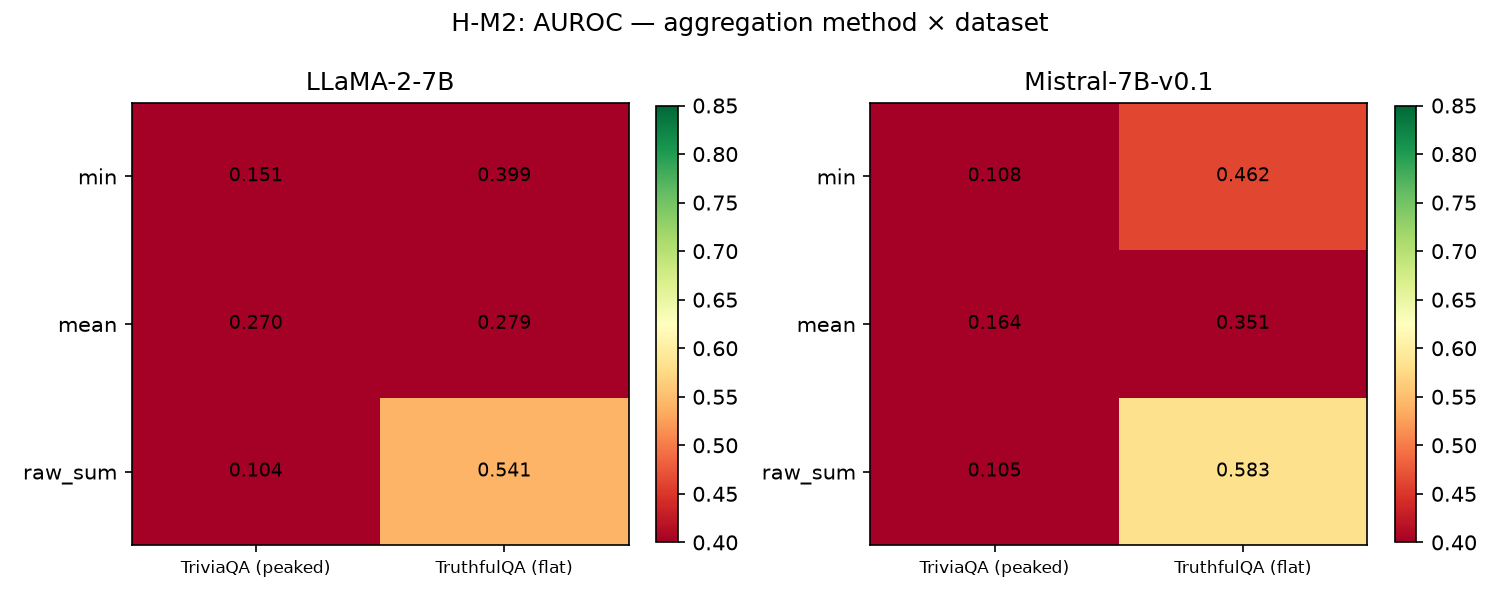
\includegraphics[width=\columnwidth]{figures/auroc_heatmap}
\caption{Full $3\times4$ AUROC heatmap across all aggregation functions and model $\times$ dataset conditions.}
\label{fig:auroc_heatmap}
\end{figure}

The consistent raw\_sum advantage across both models argues against a dataset-specific artifact and suggests sequence-level joint probability as an underexplored zero-cost factual-recall signal.
